\documentclass[11pt]{exam}
\usepackage{amsfonts,amsthm,amsmath,amssymb,mathrsfs,bbm,dsfont,bm,hyperref}
\usepackage{csquotes}\MakeOuterQuote{"}
\usepackage{hyperref}
\setlength{\paperheight}{12in}
\setlength\parindent{0pt}
\usepackage{xcolor}
\parskip=5pt 
\usepackage{scrextend}
\usepackage{graphicx}
\usepackage{anyfontsize}
\usepackage[shortlabels]{enumitem}


\qformat{\textbf{Problem \thequestion}\quad (\thepoints)\hfill}

\hypersetup{
  colorlinks=true,
  linkcolor=blue!50!red,
  urlcolor=blue!70!black
}


\begin{document}


\begin{center}

     \textbf{Bi/BE/CS 183 2022-2023\\ Instructor: Lior Pachter\\ TAs: Tara Chari, Meichen Fang, Zitong (Jerry) Wang \vskip 0.15in Problem Set 1}

\end{center}


 \vskip 0.15in


Submit your solutions as a single PDF file via Canvas by {\bf 8am Tuesday January 17th}. 
\begin{itemize}
  \item If writing up problems by hand, please use a pen and not a pencil, as it is difficult to read scanned submission of pencil work. Typed solutions are preferred.
  \item For problems that require coding, Colab notebooks will be provided. Please copy and save the shared notebook and edit your own copy, which you should then submit by including a clickable link in your submitted homework. Prior to submission make sure that you code runs from beginning to end without any error reports.
  
  See the class \href{https://caltech.instructure.com/courses/5055}{Intro to Colab} on how to produce a shareable link for your notebook.

\end{itemize}

\begin{questions}
\question[18]

Single-cell RNA sequencing (single-cell RNA-seq or scRNA-seq) technologies utilize numerous recent technology breakthroughs. While many popular methods utilize similar ideas, such as barcoding transcripts to inform on their cell of origin, there are many ways to achieve this as discussed in Lecture. \\

Briefly answer each question below:
\begin{parts} 
\part[2] What is the role of the unique molecular identifier (UMI)? 
\part[2] What is the `library' produced by single-cell sequencing methods?
\part[6] Which droplet-based method demonstrates `sub-Poisson' loading of cells per droplet? What does `sub-Poisson' mean and how is this achieved in this technology?
\part[2] What does 3' capture refer to  (as in  3' sequencing methods) ? 
\part[6] For 3' 10X sequencing, write the order in which the events below are executed for generating the final, sequenced library.
\begin{itemize}
  \item cDNA fragmentation and size selection
  \item Cell capture and lysis
  \item 3' transcript capture and barcoding
  \item Reverse transcription and amplification
  \item Addition of sample index/label (sample index PCR)
  \item Single- or paired-end sequencing

\end{itemize}

\end{parts} 

\newpage
\question[46]

Consider the following gene expression matrix $G$, containing the expression level of four genes across three cells. The $i$-th row of $G$ represents the expression level of all genes in the $i$-th cell, and the $j$-th column represents the expression level of the $j$-th gene across all cells.

\[ 
G = \begin{bmatrix}
1 & 2 & 3 & 3 \\
3 & 1 & 9 & 4 \\
1 & 4 & 3 & 5 \\
\end{bmatrix}.  
\]
 A \href{https://github.com/pachterlab/Bi-BE-CS-183-2023/blob/main/HW1/Problem2.ipynb}{Colab notebook} has been created to help with computation if needed. Note that when submitting your homework you must submit a link to a copy of this notebook if you use and modify it.
\vspace{0.1pt}
\begin{parts} 
\part[2] Which cell has the highest expression level of gene 2 (index starts from 1)? 
\part[2] Which gene is most highly expressed in cell 2?

\part One of the most fundamental characteristics of a matrix $A$ is its rank, which corresponds to the maximal number of linearly independent columns/rows of $A$. A set of vectors $\mathbf{v}_1,\mathbf{v}_2,\ldots,\mathbf{v}_n$ are linearly independent if the equation
\begin{equation*}
    a_{1} \mathbf{v}_{1}+a_{2} \mathbf{v}_{2}+\cdots+a_{n} \mathbf{v}_{n}=\mathbf{0}
\end{equation*}
can only be satisfied by $a_i = 0$ for $i=1,\ldots,n$.

\begin{subparts}
\subpart[2] Find the rank of $G$
\subpart[2] What does the rank of $G$ suggest in terms of the relationship in expression level between the four genes?
\end{subparts}

\part Suppose you are interested in selecting only highly expressed genes for further analysis. 
\begin{subparts}
\subpart[2] Find a vector $v$ such that the product $v^TG$ contains the mean expression level for every gene in $G$.
\subpart[2]	Find the mean expression level for each gene in $G$.
\subpart[4] Find a matrix $P$, such that $GP$ is a new gene expression matrix that contains, for each cell, only the expression level of the two genes with the highest mean expression.
\end{subparts}

\part In many practical applications, we are often interested in finding cells that are "similar" to one another in terms of their gene expression profiles, where the gene expression profile of a cell corresponds to a row vector of the gene expression matrix. Finding how similar two cells are amounts to computing how "close" their corresponding expression vectors are under a particular distance function.
\begin{subparts}
\subpart[9] Consider three valid distance functions between a pair of vectors $\mathbf{x}$ and $\mathbf{y}$, the $L_1$ distance, $L_2$ distance, and cosine similarity ($c$),
\begin{equation*}
	L_1(\mathbf{x},\mathbf{y}) := \| \mathbf{x} - \mathbf{y}\|_1 = \sum_{i=1}^n |x_i-y_i|,
\end{equation*}
\begin{equation*}
	L_2(\mathbf{x},\mathbf{y}) := \| \mathbf{x} - \mathbf{y}\|_2 = \sqrt{\sum_{i=1}^n (x_i-y_i)^2},
\end{equation*}
\begin{equation*}
	c(\mathbf{x},\mathbf{y}) := \frac{\mathbf{x} \cdot \mathbf{y}}{\|\mathbf{x}\|_2 \|\mathbf{y}\|_2}=\frac{\sum_{i=1}^{n} x_{i} y_{i}}{\sqrt{\sum_{i=1}^{n} x_{i}^{2}} \sqrt{\sum_{i=1}^{n} y_{i}^{2}}}.
\end{equation*}

Note that the cosine similarity is simply a measure of the cosine of the angle between two vectors. For each distance function above, construct a distance matrix $D$, where $D_{ij}$ denotes the distance between the $i$-th and $j$-th row/cell of $G$. 
\subpart[3] For each distance function, which two cells in $G$ are most similar to one another? For $L_1$ and $L_2$ distance, this corresponds to a pair of row vectors with the smallest distance, whereas for the cosine similarity, this corresponds to a pair of row vectors with the smallest angle. 
\end{subparts}

\part[9] Suppose the cell sample in an experiment has been contaminated, such that the expression level of all genes across all cells  were measured to be higher than their actual value by a constant amount. Explain (with proof) whether any of the distance functions in the previous part are affected by this contamination. 

\part[9] When comparing the gene expression profile of different cells, it may be useful to compare the relative gene expression level instead of absolute expression level (consider trying to identify same cell types from cells pooled from different growth condition). In such a case, we want to use a distance function $f$ that is invariant to scaling. Specifically, we would like $f$ to satisfy the property that for any scaling constants $a\geq 0$ and $b\geq 0$,
\[ f(\mathbf{x},\mathbf{y}) = f(a\mathbf{x},b\mathbf{y}). \]
Show that the cosine similarity satisfies this property, while the $L_1$ and $L_2$ distances do not.



\end{parts}

\newpage
\question[36]

 For this problem you will be exploring the phenomenon known as Simpson's Reversal in a single-cell sequencing dataset. \href{https://github.com/pachterlab/Bi-BE-CS-183-2023/blob/main/HW1/Problem3.ipynb}{Problem 3 Google Colab notebook here}. 
 
 As described in Lecture, Simpson's Reversal describes the phenomenon where a certain trend appears within certain groups of the data, but disappears or is reversed when the groupings are changed. This is not limited to only a `reversal', i.e. this includes a positive or negative trend in one grouping, which disappears with another grouping. \\
 
 One of the advantages of single-cell RNA sequencing as opposed to bulk RNA sequencing (where all reads from all cells are pooled together) is that it provides the opportunity, in principle, to avoid incorrect inferences about correlation between pairs of genes. \\
 
  \begin{figure}[!hb]
        \centering
        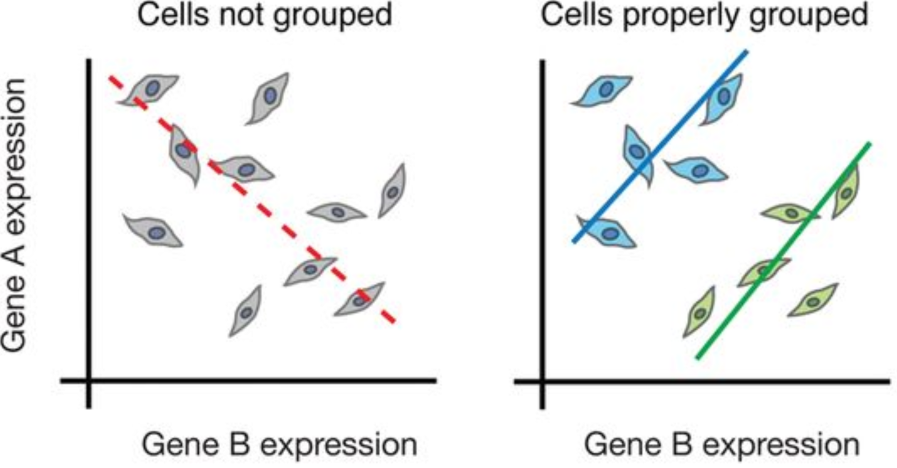
\includegraphics[scale=0.5]{Figures/groupings.png}
        \caption{Hypothetical situation in which the relationship between expression values of genes A and B differs in grouped versus not grouped cells. Figure from \cite{Trapnell2015}. }
    \end{figure}
 
 In the conceptual figure shown above, genes A and B display a negative correlation in their expression values in the bulk scenario (`Cells not grouped'). However, once the cells are grouped by their respective cell types, we see that genes A and B are positively correlated in each group (`Cells properly grouped'), though both genes are expressed at lower amounts in the green cell type. Thus, in this hypothetical scenario, single-cell resolution that facilitates resolution of the different cell populations is necessary to understand the relationship between genes A and B. \\
 
 For this problem you will mine a single-cell RNA-seq dataset to see if this phenomenon occurs in practice. Instructions are provided in the problem Colab notebook.\\

Your edited version of the notebook \textit{must be submitted } for this problem. Please remember to check that your notebook runs from the beginning to the end without reporting errors by running it with the {\tt Runtime} $\xrightarrow{}$ {\tt Restart} and {\tt Runtime} $\xrightarrow{}$ {\tt Run All} commands.\\


For help reviewing basic Python functions and coding practices see our \href{https://github.com/pachterlab/Bi-BE-CS-183-2023/blob/main/HW1/pythonReview.ipynb}{Python review notebook}.  \\



\end{questions}
\begin{thebibliography}{1}
\bibitem{Trapnell2015}
Trapnell, C., 2015. Defining cell types and states with single-cell genomics. {\it Genome research}, 25(10), pp.1491-1498.
\end{thebibliography}
\end{document}


